\chapter{FieldConvert}
\label{s:utilities:fieldconvert}
FieldConvert is a utility embedded in \nekpp with the primary aim of allowing
the user to convert the \nekpp output binary files (\inltt{.chk} and
\inltt{.fld}) into formats which can be read by common visualisation and
post-processing software, primarily Paraview/VisIt (in unstructured VTK
\inltt{.vtu} format) or Tecplot/VisIt (in ASCII \inltt{.dat} or binary
\inltt{.plt} formats). FieldConvert also allows the user to manipulate the
\nekpp output binary files by using some additional modules which can be called
with the option \inltt{-m} which stands for \inltt{m}odule. Note that another
flag, \inltt{-r} (which stand for \inltt{r}ange) allows the user to specify a
sub-range of the domain on which the conversion or manipulation of the \nekpp
output binary files will be performed.

Almost all of the FieldConvert functionalities can be run in parallel if \nekpp
is compiled using MPI (see the installation documentation for additional info on
how to implement \nekpp using MPI). \footnote{Modules that do not have parallel
  support will be specified in the appropriate section.}
%
%
%
\section{Basic usage}
FieldConvert expects at least one input specification (such as a session file
and its corresponding field file) and one output specification. These are
specified on the command line as
%
\begin{lstlisting}[style=BashInputStyle]
  FieldConvert in1.xml in2.fld out.dat
\end{lstlisting}
%
These can be combined with a processing module by adding the \inltt{-m} command
line option. There can be more than one module specified, and they can appear
anywhere in the command line arguments, although the order of execution is
inferred from their order in the command line. For example, the command
%
\begin{lstlisting}[style=BashInputStyle]
  FieldConvert in1.xml -m module1 in2.fld -m module2 out.dat
\end{lstlisting}
%
causes \inltt{in1.xml} and \inltt{in2.fld} to be read, followed by the
\inltt{module1} processing module, the \inltt{module2} processing module, and
finally output to the \inltt{out.dat} Tecplot file.

\subsection{Input formats}

FieldConvert supports XML and FLD-format files as produced by \nekpp. It also
supports the reading of data files from two external spectral element codes:
\emph{Semtex}\footnote{http://users.monash.edu.au/~bburn/semtex.html} and
\emph{Nek5000}\footnote{https://nek5000.mcs.anl.gov}. These files can be
directly converted to \nekpp format files by using the command
%
\begin{lstlisting}[style=BashInputStyle]
  FieldConvert input.fld output.fld
\end{lstlisting}
%
Note that even though the \inltt{.fld} extension is typically associated with
\nekpp files, FieldConvert can automatically identify \emph{Semtex} and
\emph{Nek5000} input field files.

To use these files in a simulation, or to post-process the results of a
simulation, an appropriate mesh must also be defined in the \nekpp XML format.
\nm can be used to convert these input files to XML, as outlined in
section~\ref{s:utilities:nekmesh}.

\section{Convert .fld / .chk files into Paraview, VisIt or Tecplot format}
\label{s:utilities:fieldconvert:sub:convert}
To convert the \nekpp output binary files (.chk and .fld) into a
format which can be read by two common visualisation softwares:
Paraview (.vtu format), VisIt (.vtu format) or Tecplot (.dat or .plt format)
the user can run the following commands:
%
\begin{itemize}
\item Paraview or VisIt (.vtu format)
%
\begin{lstlisting}[style=BashInputStyle]
FieldConvert test.xml test.fld test.vtu
\end{lstlisting}
%
\item Tecplot (.dat format)
%
\begin{lstlisting}[style=BashInputStyle]
FieldConvert test.xml test.fld test.dat
\end{lstlisting}
%
\item Tecplot or VisIt(.plt format)
%
\begin{lstlisting}[style=BashInputStyle]
FieldConvert test.xml test.fld test.plt
\end{lstlisting}
\end{itemize}
%
where \inltt{FieldConvert} is the executable associated to the utility
FieldConvert, \inltt{test.xml} is the session file and
\inltt{test.vtu}, \inltt{test.dat},  \inltt{test.plt} are the desired
format outputs, either Paraview, VisIt or Tecplot formats. \\
When converting to \inltt{.dat} or \inltt{.plt} format, it is possible to
enable output with double precision, which is more accurate but requires larger
disk space. For example, double precision output in plt. format can be produced
with the command:
\begin{lstlisting}[style=BashInputStyle]
FieldConvert test.xml test.fld test.plt:plt:double
\end{lstlisting}
%
\begin{tipbox}
Note that the session file is also supported
in its compressed format \inltt{test.xml.gz}.
\end{tipbox}
%
%
%
\section{Convert field files between XML and HDF5 format}
%
When \nekpp is compiled with HDF5 support, solvers can select the format used
for output of \inltt{.fld} files. FieldConvert can be used to convert between
these formats using an option on the \inltt{.fld} output module. For example, if
\inltt{in.fld} is stored in the default XML format, it can be converted to HDF5
format by issuing the command
%
\begin{lstlisting}[style=BashInputStyle]
FieldConvert in.fld out.fld:fld:format=Hdf5
\end{lstlisting}
%
\section{Range option \textit{-r}}
The Fieldconvert range option \inltt{-r} allows the user to specify
a sub-range of the mesh (computational domain) by using an
additional flag, \inltt{-r} (which stands for \inltt{r}ange and either
convert or manipulate the \nekpp output binary files.
Taking as an example the conversion of the \nekpp binary files
(.chk or .fld) shown before and wanting to convert just the 2D
sub-range defined by $-2\leq x \leq 3$, $-1\leq y \leq 2$ the
additional flag \inltt{-r} can be used as follows:
%
\begin{itemize}
\item Paraview or VisIt (.vtu format)
%
\begin{lstlisting}[style=BashInputStyle]
FieldConvert -r -2,3,-1,2 test.xml test.fld test.vtu
\end{lstlisting}
%
\item Tecplot (.dat format)
%
\begin{lstlisting}[style=BashInputStyle]
FieldConvert -r 2,3,-1,2 test.xml test.fld test.dat
\end{lstlisting}
%
\end{itemize}
where \inltt{-r} defines the range option of the FieldConvert
utility, the two first numbers define the range in $x$ direction
and the the third and fourth number specify the $y$ range.
A sub-range of a 3D domain can also be specified.
For doing so, a third set of numbers has to be provided
to define the $z$ range.
%
%
%

\section{FieldConvert in NekPy}

The Python interface allows the user to instantiate input,
output, and process modules by calling the static \verb+Create+ method of the
\verb+InputModule+, \verb+ProcessModule+, and \verb+OutputModule+,
register configuration options, and run them.
For example, consider the command:

\begin{lstlisting}[style=BashInputStyle]
FieldConvert -n 10 -m wss:bnd=0 session.xml field.fld  field_wss.fld
\end{lstlisting}


A Python script performing the same task is given below.

\begin{lstlisting}[style=C++Style, language=Python]
import sys
from NekPy.FieldUtils import *

field = Field(sys.argv, output_points=10)

InputModule.Create("xml",   field, "session.xml").Run()
InputModule.Create("fld",   field, "field.fld").Run()
ProcessModule.Create("wss", field,  bnd="0").Run()
OutputModule.Create("fld" , field, "field_wss.fld").Run()
\end{lstlisting}

The key points are that the FieldConvert command line options, in this
case \inltt{output-points}, are passed to the constructor of \verb+Field+.
The configuration options for a given module are passed to the static
\verb+Create+ method of the \verb+InputModule+, \verb+ProcessModule+, and
\verb+OutputModule+. This creates the corresponding module and the
modules can be run immediately after instantiation. Note that the first
parameter of the \verb+Create+ method has to be the key for a given module,
the second is the field variable and for input and output modules the remaining
arguments may identify the input and output files for a given module.
Optionally we can explicitly specify the file type of an input module
using the "infile" keyword and the "outfile" keyword for output modules.


\begin{lstlisting}[style=C++Style, language=Python]
import sys
from NekPy.FieldUtils import *

field = Field(sys.argv, output_points=10)

InputModule.Create("xml",   field, infile={"xml": "session.xml"}).Run()
InputModule.Create("fld",   field, infile={"fld": "field.fld"}).Run()
ProcessModule.Create("wss", field, bnd="0").Run()
OutputModule.Create("fld" , field, outfile="field_wss.fld").Run()
\end{lstlisting}

It can also emulate the functionality of FieldConvert when using the
\inltt{nparts} option in the following way. Here \verb+session_xml+ is a
directory containing the mesh partitioned into 2.

\begin{lstlisting}[style=C++Style, language=Python]
import sys
from NekPy.FieldUtils import *

field = Field(sys.argv, nparts=2, forceoutput=True, error=True)

inputxml   = InputModule.Create("xml",   field, "session_xml")
inputfld   = InputModule.Create("fld",   field, "field.fld")
processwss = ProcessModule.Create("wss", field,  bnd="2")
outputfld  = OutputModule.Create("fld",  field, "field_wss.fld")

for part in range(2):
	field.NewPartition(sys.argv, part)
	inputxml.Run()
	inputfld.Run()
	processwss.Run()
	outputfld.Run()

OutputModule.Create("info", field, "field_wss_b0.fld", nparts=2).Run()
\end{lstlisting}

The number of partitions is looped over, with \verb+NewPartition+ called at
the start of each. When using \verb+OutputModule+, the \verb+info+ module
must be used in order to obtain the correct result.

\section{FieldConvert modules \textit{-m}}
FieldConvert allows the user to manipulate the \nekpp output
binary files (.chk and .fld) by using the flag \inltt{-m} (which
stands for \inltt{m}odule).
Specifically, FieldConvert has these additional functionalities
%
\begin{enumerate}
\item \inltt{C0Projection}: Computes the C0 projection of a given output file;
\item \inltt{QCriterion}: Computes the Q-Criterion for a given output file;
\item \inltt{L2Criterion}: Computes the Lambda 2 Criterion for a given output file;
\item \inltt{addcompositeid}: Adds the composite ID of an element as an additional field;
\item \inltt{fieldfromstring}: Modifies or adds a new field from an expression involving the existing fields;
\item \inltt{addFld}: Sum two .fld files;
\item \inltt{combineAvg}: Combine two \nekpp binary output (.chk or .fld) field file containing averages of fields (and
possibly also Reynolds stresses) into single file;
\item \inltt{concatenate}: Concatenate a \nekpp binary output (.chk or .fld) field file into single file (deprecated);
\item \inltt{dof}: Count the total number of DOF;
\item \inltt{equispacedoutput}: Write data as equi-spaced output using simplices to represent the data for connecting points;
\item \inltt{extract}: Extract a boundary field;
\item \inltt{gradient}: Computes gradient of fields;
\item \inltt{halfmodetofourier}: Convert \inltt{HalfMode} expansion to \inltt{SingleMode} for further processing;
\item \inltt{homplane}: Extract a plane from 3DH1D expansions;
\item \inltt{homstretch}: Stretch a 3DH1D expansion by an integer factor;
\item \inltt{innerproduct}: take the inner product between one or a series of fields with another field (or series of fields).
\item \inltt{interpfield}: Interpolates one field to another, requires fromxml, fromfld to be defined;
\item \inltt{interppointdatatofld}: Interpolates given discrete data using a finite difference approximation to a fld file given an xml file;
\item \inltt{interppoints}: Interpolates a field to a set of points. Requires fromfld, fromxml to be defined, and a topts, line, plane or box of target points;
\item \inltt{interpptstopts}: Interpolates a set of points to another. Requires a topts, line, plane or box of target points;
\item \inltt{isocontour}: Extract an isocontour of ``fieldid'' variable and at value ``fieldvalue''. Optionally ``fieldstr'' can be specified for a string definition or ``smooth'' for smoothing;
\item \inltt{jacobianenergy}: Shows high frequency energy of Jacobian;
\item \inltt{qualitymetric}: Evaluate a quality metric of the underlying mesh to show mesh quality;
\item \inltt{mean}: Evaluate the mean of variables on the domain;
\item \inltt{meanmode}: Extract mean mode (plane zero) of 3DH1D expansions;
\item \inltt{pointdatatofld}: Given discrete data at quadrature points
  project them onto an expansion basis and output fld file;
\item \inltt{printfldnorms}: Print L2 and LInf norms to stdout;
\item \inltt{removefield}: Removes one or more fields from .fld files;
\item \inltt{scalargrad}: Computes scalar gradient field;
\item \inltt{scaleinputfld}: Rescale input field by a constant factor;
\item \inltt{shear}: Computes time-averaged shear stress metrics: TAWSS, OSI, transWSS, TAAFI, TACFI, WSSG;
\item \inltt{streamfunction}: Calculates stream function of a 2D incompressible flow.
\item \inltt{surfdistance}: Computes height of a prismatic boundary layer mesh and projects onto the surface (for e.g. $y^+$ calculation).
\item \inltt{vorticity}: Computes the vorticity field.
\item \inltt{wss}: Computes wall shear stress field.
\item \inltt{phifile}: Computes the $\Phi$ function representing a body defined
  in an \inltt{.stl} file. Useful for the Smoothed Profile Method solver.
\item \inltt{wallNormalData}: Interpolate values for a set of points in the wall-normal direction (for e.g. extract boundary layer profiles).
\end{enumerate}
The module list above can be seen by running the command
%
\begin{lstlisting}[style=BashInputStyle]
FieldConvert -l
\end{lstlisting}
%
In the following we will detail the usage of each module.
%
%
%

\subsection{Smooth the data: \textit{C0Projection} module}
To smooth the data of a given .fld file one can
use the \inltt{C0Projection} module of FieldConvert
%
\begin{lstlisting}[style=BashInputStyle]
FieldConvert -m C0Projection test.xml test.fld test-C0Proj.fld
\end{lstlisting}
%
where the file \inltt{test-C0Proj.fld} can be processed in a similar
way as described in section \ref{s:utilities:fieldconvert:sub:convert}
to visualise the result either in Tecplot, Paraview or VisIt.

The option \inltt{localtoglobalmap} will do a global gather of the
coefficients and then scatter them back to the local elements. This
will replace the coefficients shared between two elements with the
coefficients of one of the elements (most likely the one with the
highest id). Although not a formal projection it does not require any
matrix inverse and so is very cheap to perform.

The option \inltt{usexmlbcs} will enforce the boundary conditions
specified in the input xml file.

The option \inltt{helmsmoothing=$L$} will perform a Helmholtz
smoothing projection of the form
\[
\left (\nabla^2 - \left (\frac{2 \pi}{L}\right )^2 \right ) \hat{u}^{new} =
-\left (\frac{2 \pi}{L}\right )^2 \hat{u}^{orig}
\]
which can be interpreted in a Fourier sense as smoothing the original
coefficients using a low pass filter of the form
\[
\hat{u}_k^{new} = \frac{1}{(1 + k^2/K_0^2)} \hat{u}_k^{orig} \mbox{\,  where  \,}
K_0 = \frac{2 \pi}{L}
\]
and so $L$ is the length scale below which the coefficients values are
halved or more. Since this form of the Helmholtz operator is not
possitive definite, currently a direct solver is necessary and so this
smoother is mainly of use in two-dimensions.

\subsection{Calculate Q-Criterion: \textit{QCriterion} module}
To perform the Q-criterion calculation and obtain an output
data containing the Q-criterion solution, the user can run
%
\begin{lstlisting}[style=BashInputStyle]
FieldConvert -m QCriterion test.xml test.fld test-QCrit.fld
\end{lstlisting}
%
where the file \inltt{test-QCrit.fld} can be processed in a similar
way as described in section \ref{s:utilities:fieldconvert:sub:convert}
to visualise the result either in Tecplot, Paraview or VisIt.
%
%
%

\subsection{Calculate $\lambda_2$: \textit{L2Criterion} module}
To perform the $\lambda_2$ vortex detection calculation and obtain an output
data containing the values of the $\lambda_2$ eigenvalue, the user can run
%
\begin{lstlisting}[style=BashInputStyle]
  FieldConvert -m L2Criterion test.xml test.fld test-L2Crit.fld
\end{lstlisting}
%
where the file \inltt{test-L2Crit.fld} can be processed in a similar
way as described in section \ref{s:utilities:fieldconvert:sub:convert}
to visualise the result either in Tecplot, Paraview or VisIt.
%
%
%

\subsection{Add composite ID: \textit{addcompositeid} module}
When dealing with a geometry that has many surfaces, we need to identify the
composites to assign boundary conditions. To assist in this, FieldConvert has a
\inltt{addcompositeid} module, which adds the composite ID of every element as a
new field. To use this we simply run
%
\begin{lstlisting}[style=BashInputStyle]
  FieldConvert -m addcompositeid mesh.xml out.dat
\end{lstlisting}
%
In this case, we have produced a Tecplot file which contains the mesh and a
variable that contains the composite ID. To assist in boundary identification,
the input file \inlsh{mesh.xml} should be a surface XML file that can be
obtained through the \nm \inltt{extract} module (see section
\ref{s:utilities:nekmesh:extract}).
%
%
%
\subsection{Add new field: \textit{fieldfromstring} module}
To modify or create a new field using an expression involving the existing fields, one can
use the \inltt{fieldfromstring} module of FieldConvert
%
\begin{lstlisting}[style=BashInputStyle]
  FieldConvert -m fieldfromstring:fieldstr="x+y+u":fieldname="result" \
  file1.xml file2.fld file3.fld
\end{lstlisting}
%
In this case \inltt{fieldstr} is a required parameter describing a function of
the coordinates and the existing variables, and \inltt{fieldname} is an optional
parameter defining the name of the new or modified field (the default is newfield).
\inltt{file3.fld} is the output containing both the original and the new fields,
and can be processed in a similar way as described
in section \ref{s:utilities:fieldconvert:sub:convert} to visualise
the result either in Tecplot, Paraview or VisIt.
%
%
%
\subsection{Sum two .fld files: \textit{addFld} module}
To sum two .fld files one can use the \inltt{addFld} module of FieldConvert
%
\begin{lstlisting}[style=BashInputStyle]
  FieldConvert -m addfld:fromfld=file1.fld:scale=-1 file1.xml file2.fld \
  file3.fld
\end{lstlisting}
%
In this case we use it in conjunction with the command \inltt{scale}
which multiply the values of a given .fld file by a constant \inltt{value}.
\inltt{file1.fld} is the file multiplied by \inltt{value}, \inltt{file1.xml}
is the associated session file, \inltt{file2.fld} is the .fld file which
is summed to \inltt{file1.fld} and finally \inltt{file3.fld} is the output
which contain the sum of the two .fld files.
\inltt{file3.fld} can be processed in a similar way as described
in section \ref{s:utilities:fieldconvert:sub:convert} to visualise
the result either in Tecplot, Paraview or VisIt.
%
%
%
\subsection{Combine two .fld files containing time averages: \textit{combineAvg} module}
To combine two .fld files obtained through the AverageFields or ReynoldsStresses filters,
use the \inltt{combineAvg} module of FieldConvert
%
\begin{lstlisting}[style=BashInputStyle]
  FieldConvert -m combineAvg:fromfld=file1.fld file1.xml file2.fld \
  file3.fld
\end{lstlisting}
%
\inltt{file3.fld} can be processed in a similar way as described
in section \ref{s:utilities:fieldconvert:sub:convert} to visualise
the result either in Tecplot, Paraview or VisIt.
%
%
%
\subsection{Concatenate two files: \textit{concatenate} module}
To concatenate \inltt{file1.fld} and \inltt{file2.fld} into \inltt{file-conc.fld}
one can run the following command
%
\begin{lstlisting}[style=BashInputStyle]
FieldConvert file.xml  file1.fld  file2.fld  file-conc.fld
\end{lstlisting}
%
where the file \inltt{file-conc.fld} can be processed in a similar
way as described in section \ref{s:utilities:fieldconvert:sub:convert}
to visualise the result either in Tecplot, Paraview or VisIt. The
\inltt{concatenate} module previously used for this purpose is not
required anymore, and will be removed in a future release.
%
%
%
\subsection{Count the number of DOF: \textit{dof} module}
To count the number of DOF in a solution file,
one can run the following command
%
\begin{lstlisting}[style=BashInputStyle]
FieldConvert -m dof file.xml file.fld out.stdout
\end{lstlisting}
%
%
%
\subsection{Equi-spaced output of data: \textit{equispacedoutput} module}
This module interpolates the output data to a truly equispaced set of
points (not equispaced along the collapsed coordinate
system). Therefore a tetrahedron is represented by a tetrahedral
number of poinst. This produces much smaller output files. The points
are then connected together by simplices (triangles and tetrahedrons).

\begin{lstlisting}[style=BashInputStyle]
FieldConvert -m equispacedoutput test.xml test.fld test.dat
\end{lstlisting}

or

\begin{lstlisting}[style=BashInputStyle]
FieldConvert -m equispacedouttput test.xml test.fld test.vtu
\end{lstlisting}


\begin{notebox}
Currently this option is only set up for triangles, quadrilaterals,
tetrahedrons and prisms.
\end{notebox}

\subsection{Extract a boundary region: \textit{extract} module}
The boundary region of a domain can be extracted from the output
data using the following command line
%
\begin{lstlisting}[style=BashInputStyle]
FieldConvert -m extract:bnd=2 test.xml \
	test.fld test-boundary.fld
\end{lstlisting}
%
The option \inltt{bnd} specifies which boundary region to extract.
Note this is different to NekMesh where the parameter \inltt{surf}
is specified and corresponds to composites rather boundaries. If \inltt{bnd}
is not provided, all boundaries are extracted to different fields.
The output will be placed in test-boundary\_b2.fld.
If more than one boundary region is specified the extension \_b0.fld, \_b1.fld etc will be
outputted. To process this file you will need an xml file of the same region.
This can be generated using the command:
%
\begin{lstlisting}[style=BashInputStyle]
NekMesh -m extract:surf=5  test.xml test\_b0.xml
\end{lstlisting}
%
The surface to be extracted in this command is the composite
number and so needs to correspond to the boundary region
of interest. Finally to process the surface file one can use
%
\begin{lstlisting}[style=BashInputStyle]
FieldConvert  test\_b0.xml test\_b0.fld test\_b0.dat
\end{lstlisting}
%
This will obviously generate a Tecplot output if a .dat file
is specified as last argument. A .vtu extension will produce
a Paraview or VisIt output.
%
%
%
\subsection{Compute the gradient of a field: \textit{gradient} module}
To compute the spatial gradients of all fields one can run the following command
%
\begin{lstlisting}[style=BashInputStyle]
FieldConvert -m gradient test.xml  test.fld  test-grad.fld
\end{lstlisting}
%
where the file \inltt{file-grad.fld} can be processed in a similar
way as described in section \ref{s:utilities:fieldconvert:sub:convert}
to visualise the result either in Tecplot, Paraview or VisIt.
%
%

\subsection{Convert HalfMode expansion to SingleMode for further processing: \textit{halfmodetofourier} module}

To obtain full Fourier expansion form a \inltt{HalfMode} result, use the comand:
\begin{lstlisting}[style=BashInputStyle]
  FieldConvert -m halfmodetofourier file.xml half_mode_file.fld single_mode_file.fld
\end{lstlisting}

\subsection{Extract a plane from 3DH1D expansion: \textit{homplane} module}

To obtain a 2D expansion containing one of the planes of a
3DH1D field file, use the command:
\begin{lstlisting}[style=BashInputStyle]
FieldConvert -m homplane:planeid=value file.xml file.fld file-plane.fld
\end{lstlisting}

If the option \inltt{wavespace} is used, the Fourier coefficients
corresponding to \inltt{planeid} are obtained. The command in this case is:
\begin{lstlisting}[style=BashInputStyle]
FieldConvert -m homplane:wavespace:planeid=value file.xml \
    file.fld file-plane.fld
\end{lstlisting}

The output file \inltt{file-plane.fld} can be processed in a similar
way as described in section \ref{s:utilities:fieldconvert:sub:convert}
to visualise it either in Tecplot or in Paraview.

\subsection{Stretch a 3DH1D expansion: \textit{homstretch} module}

To stretch a 3DH1D expansion in the z-direction, use the command:
\begin{lstlisting}[style=BashInputStyle]
FieldConvert -m homstretch:factor=value file.xml file.fld file-stretch.fld
\end{lstlisting}
The number of modes in the resulting field can be chosen using the command-line
parameter \inltt{-{}-output-points-hom-z}.

The output file \inltt{file-stretch.fld} can be processed in a similar
way as described in section \ref{s:utilities:fieldconvert:sub:convert}
to visualise it either in Tecplot or in Paraview.


\subsection{Inner Product of a single or series of fields with respect to a single or series of fields: \textit{innerproduct} module}
You can take the inner product of one field with another field using
the following command:
\begin{lstlisting}[style=BashInputStyle]
  FieldConvert -m innerproduct:fromfld=file1.fld  file2.xml file2.fld \
  out.stdout
\end{lstlisting}
This command will load the \inltt{file1.fld} and \inltt{file2.fld}
assuming they both are spatially defined by \inltt{files.xml} and
determine the inner product of these fields. The input option
\inltt{fromfld} must therefore be specified in this module.

Optional arguments for this module are \inltt{fields} which allow you to specify
the fields that you wish to use for the inner product, i.e.
\begin{lstlisting}[style=BashInputStyle]
  FieldConvert -m innerproduct:fromfld=file1.fld:fields="0,1,2" file2.xml \
  file2.fld out.stdout
\end{lstlisting}
will only take the inner product between the variables 0,1 and 2 in
the two fields files. The default is to take the inner product between
all fields provided.

Additional options include \inltt{multifldids} and \inltt{allfromflds}
which allow for a series of fields to be evaluated in the following
manner:
\begin{lstlisting}[style=BashInputStyle]
  FieldConvert -m innerproduct:fromfld=file1.fld:multifldids="0-3"\
  file2.xml  file2.fld out.stdout
\end{lstlisting}
will take the inner product between a file names
field1\_0.fld, field1\_1.fld, field1\_2.fld and field1\_3.fld with
respect to field2.fld.

Analogously including the options \inltt{allfromflds}, i.e.
\begin{lstlisting}[style=BashInputStyle]
  FieldConvert -m innerproduct:fromfld=file1.fld:multifldids="0-3":\
  allfromflds  file2.xml file2.fld out.stdout
\end{lstlisting}
Will take the inner product of all the from fields,
i.e. field1\_0.fld,field1\_1.fld,field1\_2.fld and field1\_3.fld with
respect to each other. This option essentially ignores file2.fld. Only
the unique inner products are evaluated so if four from fields are
given only the related trianuglar number $4\times5/2=10$ of inner
products are evaluated.

This option can be run in parallel.

%
%
%

\subsection{Interpolate one field to another: \textit{interpfield} module}
To interpolate one field to another, one can use the following command:
%
\begin{lstlisting}[style=BashInputStyle]
FieldConvert -m interpfield:fromxml=file1.xml:fromfld=file1.fld \
	file2.xml file2.fld
\end{lstlisting}
%
This command will interpolate the field defined by \inltt{file1.xml}
and \inltt{file1.fld} to the new mesh defined in \inltt{file2.xml} and
output it to \inltt{file2.fld}.
The \inltt{fromxml} and \inltt{fromfld} must be specified in this module.
In addition there are two optional arguments \inltt{clamptolowervalue}
and \inltt{clamptouppervalue} which clamp the interpolation between
these two values. Their default values are -10,000,000 and 10,000,000.
%
\begin{tipbox}
This module can run in parallel where the speed is increased not
only due to using more cores but also, since the mesh is split into
smaller sub-domains, the search method currently adopted performs
faster.
\end{tipbox}
%
%
%
\subsection{Interpolate scattered point data to a field: \textit{interppointdatatofld} module}
\label{s:utilities:fieldconvert:sub:interppointdatatofld}
To interpolate discrete point data to a field, use the interppointdatatofld module:
%
\begin{lstlisting}[style=BashInputStyle]
FieldConvert -m interppointdatatofld:frompts=file1.pts file1.xml file1.fld
\end{lstlisting}
or alternatively for csv data:
 \begin{lstlisting}[style=BashInputStyle]
FieldConvert -m interppointdatatofld:frompts=file1.csv file1.xml file1.fld
\end{lstlisting}
%
This command will interpolate the data from \inltt{file1.pts} (\inltt{file1.csv}) to the mesh
and expansions defined in \inltt{file1.xml} and output the field to \inltt{file1.fld}.
The file \inltt{file.pts} must be of the form:
%
\begin{lstlisting}[style=XMLStyle]
<?xml version="1.0" encoding="utf-8" ?>
<NEKTAR>
  <POINTS DIM="1" FIELDS="a,b,c">
    1.0000 -1.0000 1.0000 -0.7778
    2.0000 -0.9798 0.9798 -0.7980
    3.0000 -0.9596 0.9596 -0.8182
    4.0000 -0.9394 0.9394 -0.8384
  </POINTS>
</NEKTAR>
\end{lstlisting}
%
where \inltt{DIM="1" FIELDS="a,b,c} specifies that the field is one-dimensional
and contains three variables, $a$, $b$, and $c$.
Each line defines a point, while the  first column contains its $x$-coordinate,
the second one contains the $a$-values, the third the $b$-values and so on.
In case of $n$-dimensional data, the $n$ coordinates are specified in the first $n$
columns accordingly.
%
An equivalent csv file is:
\begin{lstlisting}[style=BashInputStyle]
# x, a, b, c
1.0000,-1.0000,1.0000,-0.7778
2.0000,-0.9798,0.9798,-0.7980
3.0000,-0.9596,0.9596,-0.8182
4.0000,-0.9394,0.9394,-0.8384
\end{lstlisting}
%
In order to interpolate 1D data to a $n$D field, specify the matching coordinate in
the output field using the \inltt{interpcoord} argument:
%
\begin{lstlisting}[style=BashInputStyle]
FieldConvert -m interppointdatatofld:frompts=1D-file1.pts:interpcoord=1 \
        3D-file1.xml 3D-file1.fld
\end{lstlisting}
%
This will interpolate the 1D scattered point data from \inltt{1D-file1.pts} to the
$y$-coordinate of the 3D mesh defined in \inltt{3D-file1.xml}. The resulting field
will have constant values along the $x$ and $z$ coordinates.
For 1D Interpolation, the module implements a quadratic scheme and automatically
falls back to a linear method if only two data points are given.
A modified inverse distance method is used for 2D and 3D interpolation.
Linear and quadratic interpolation require the data points in the \inlsh{.pts}-file to be
sorted by their location in ascending order.
The Inverse Distance implementation has no such requirement.
%
%
%
\subsection{Interpolate a field to a series of points: \textit{interppoints} module}
You can interpolate one field to a series of given points using the following command:
\begin{lstlisting}[style=BashInputStyle]
FieldConvert -m interppoints:fromxml=file1.xml:fromfld=\
        file1.fld:topts=file2.pts file2.dat
\end{lstlisting}
This command will interpolate the field defined by \inltt{file1.xml} and
\inltt{file1.fld} to the points defined in \inltt{file2.pts} and output it to
\inltt{file2.dat}.
The \inltt{fromxml} and \inltt{fromfld} must be specified in this module.
The format of the file \inltt{file2.pts} is of the same form as for the
\textit{interppointdatatofld} module:
\begin{lstlisting}[style=XMLStyle]
<?xml version="1.0" encoding="utf-8" ?>
<NEKTAR>
  <POINTS DIM="2" FIELDS="">
    0.0 0.0
    0.5 0.0
    1.0 0.0
  </POINTS>
</NEKTAR>
\end{lstlisting}
Similar to the \textit{interppointdatatofld} module, the \inltt{.pts} file can
be interchanged with a \inltt{.csv} file (the output can also be written to
\inltt{.csv}):
\begin{lstlisting}[style=BashInputStyle]
# x, y
0.0,0.0
0.5,0.0
1.0,0.0
\end{lstlisting}

There are three optional arguments \inltt{clamptolowervalue},
\inltt{clamptouppervalue} and \inltt{defaultvalue} the first two clamp the
interpolation between these two values and the third defines the default
value to be used if the point is outside the domain. Their default values
are -10,000,000, 10,000,000 and 0.

In addition, instead of specifying the file \inltt{file2.pts}, a module list of
the form
\begin{lstlisting}[style=BashInputStyle]
FieldConvert -m interppoints:fromxml=file1.xml:fromfld= \
	file1.fld:line=npts,x0,y0,x1,y1 file2.dat
\end{lstlisting}
can be specified where \inltt{npts} is the number of equispaced points between
$(x_0,y_0)$ to $(x_1,y_1)$. This also works in 3D, by specifying
$(x_0,y_0,z_0)$ to $(x_1,y_1,z_1)$.

An extraction of a plane of points can also be specified by
\begin{lstlisting}[style=BashInputStyle]
  FieldConvert -m interppoints:fromxml=file1.xml:fromfld=file1.fld:\
        plane=npts1,npts2,x0,y0,z0,x1,y1,z1,x2,y2,z2,x3,y3,z3 file2.dat
\end{lstlisting}
where \inltt{npts1,npts2} is the number of equispaced points in each
direction and $(x_0,y_0,z_0)$, $(x_1,y_1,z_1)$, $(x_2,y_2,z_2)$ and
$(x_3,y_3,z_3)$ define the plane of points specified in a clockwise or
anticlockwise direction.

In addition, an extraction of a box of points can also be specified by
\begin{lstlisting}[style=BashInputStyle]
  FieldConvert -m interppoints:fromxml=file1.xml:fromfld=file1.fld:\
       box=npts1,npts2,npts3,xmin,xmax,ymin,ymax,zmin,zmax file2.dat
\end{lstlisting}
where \inltt{npts1,npts2,npts3} is the number of equispaced points in each
direction and $(x_{min},y_{min},z_{min})$ and $(x_{max},y_{max},z_{max})$
define the limits of the box of points.

There is also an additional optional argument \inltt{cp=p0,q} which adds to the
interpolated fields the value of $c_p=(p-p0)/q$ and $c_{p0}=(p-p0+0.5 u^2)/q$
where $p0$ is a reference pressure and $q$ is the free stream dynamics pressure.
If the input does not contain a field ``p'' or a velocity field ``u,v,w'' then $cp$
and $cp0$ are not evaluated accordingly.

Interpolation of 3DH1D fields is performed only in the x-y
spectral/\emph{hp} planes. At every x-y location, if the point lies outside a
Fourier plane its z-coordinate is reset to the closest plane.
%
\begin{notebox}
This module  runs in parallel for the line, plane and box extraction of points.
\end{notebox}
%
%
%
\subsection{Interpolate a set of points to another: \textit{interpptstopts} module}
You can interpolate one set of points to another using the following command:
\begin{lstlisting}[style=BashInputStyle]
FieldConvert file1.pts -m interpptstopts:topts=file2.pts file2.dat
\end{lstlisting}
This command will interpolate the data in  \inltt{file1.pts} to a new set
of points defined in \inltt{file2.pts} and output it to
\inltt{file2.dat}.

Similarly to the \textit{interppoints} module, the target point distribution
can also be specified using the \inltt{line}, \inltt{plane} or \inltt{box}
options. The optional arguments \inltt{clamptolowervalue},
\inltt{clamptouppervalue}, \inltt{defaultvalue} and \inltt{cp} are also
supported with the same meaning as in \textit{interppoints}.

One useful application for this module is with 3DH1D expansions, for which
currently the \textit{interppoints} module does not work. In this case, we can
use for example
\begin{lstlisting}[style=BashInputStyle]
FieldConvert file1.xml file1.fld -m interpptstopts:\
    plane=npts1,npts2,x0,y0,z0,x1,y1,z1,x2,y2,z2,x3,y3,z3 \
    file2.dat
\end{lstlisting}
With this usage, the \textit{equispacedoutput} module will be automatically
called to interpolate the field to a set of equispaced points in each element.
The result is then interpolated to a plane by the \textit{interpptstopts} module.

\begin{notebox}
	This module  does not work in parallel.
\end{notebox}

%
%
%
\subsection{Isocontour extraction: \textit{iscontour} module}

Extract an isocontour from a field file. This option automatically
take the field to an equispaced distribution of points connected by
linear simplicies of triangles or tetrahedrons. The linear simplices
are then inspected to extract the isocontour of interest. To specify
the field \inltt{fieldid} can be provided giving the id of the field
of interest and \inltt{fieldvalue} provides the value of the
isocontour to be extracted.

\begin{lstlisting}[style=BashInputStyle]
  FieldConvert -m isocontour:fieldid=2:fieldvalue=0.5 test.xml test.fld \
          test-isocontour.dat
\end{lstlisting}

Alternatively \inltt{fieldstr="u+v"} can be specified to calculate
the field $u+v$ and extract its isocontour. You can also specify
\inltt{fieldname="UplusV"} to define the name of the isocontour in
the .dat file, i.e.
\begin{lstlisting}[style=BashInputStyle]
  FieldConvert -m isocontour:fieldstr="u+v":fieldvalue=0.5:\
    fieldname="UplusV" test.xml  test.fld test-isocontour.dat
\end{lstlisting}

Optionally \inltt{smooth} can be specified to smooth the isocontour
with default values \inltt{smoothnegdiffusion}=0.495,
\inltt{smoothnegdiffusion}=0.5 and \inltt{smoothiter}=100. This option
typically should be used wiht the \inltt{globalcondense} option which
removes multiply defined verties from the simplex definition which
arise as isocontour are generated element by element. The
\inltt{smooth} option preivously automatically called the
\inltt{globalcondense} option but this has been depracated since it is
now possible to read isocontour files directly and so it is useful to
have these as separate options.

In addition to the \inltt{smooth} or \inltt{globalcondense} options
you can specify \inltt{removesmallcontour}=100 which will remove
separate isocontours of less than 100 triangles.

\begin{notebox}
Currently this option is only set up for triangles, quadrilaterals,
 tetrahedrons and prisms.
\end{notebox}
%
%
%
%

\subsection{Show high frequency energy of the Jacobian: \textit{jacobianenergy} module}

\begin{lstlisting}[style=BashInputStyle]
FieldConvert -m jacobianenergy file.xml file.fld jacenergy.fld
\end{lstlisting}

The option \inltt{topmodes} can be used to specify the number of top modes to
keep.

The output file \inltt{jacenergy.fld} can be processed in a similar
way as described in section \ref{s:utilities:fieldconvert:sub:convert}
to visualise the result either in Tecplot, Paraview or VisIt.

\subsection{Calculate mesh quality: \textit{qualitymetric} module}

The \inltt{qualitymetric} module assesses the quality of the mesh by calculating
a per-element quality metric and adding an additional field to any resulting
output. This does not require any field input, therefore an example usage looks
like

\begin{lstlisting}[style=BashInputStyle]
FieldConvert -m qualitymetric mesh.xml mesh-with-quality.dat
\end{lstlisting}

Two quality metrics are implemented that produce scalar fields $Q$:

\begin{itemize}
  \item By default a metric outlined in~\cite{GaRoPeSa15} is produced, where all
  straight sided elements have quality $Q = 1$ and $Q < 1$ shows the deformation
  between the curved element and the straight-sided element. If $Q = 0$ then the
  element is invalid. Note that $Q$ varies over the volume of the element but is
  not guaranteed to be continuous between elements.
  \item Alternatively, if the \inlsh{scaled} option is passed through to the
  module, then the scaled Jacobian
  \[
    J_s =
    \frac{\min_{\xi\in\Omega_{\text{st}}}J(\xi)}{\max_{\xi\in\Omega_{\text{st}}}J(\xi)}
  \]
  (i.e. the ratio of the minimum to maximum Jacobian of each element) is
  calculated. Again $Q = 1$ denotes an ideal element, but now invalid elements
  are shown by $Q < 0$. Any elements with $Q$ near zero are determined to be low
  quality.
\end{itemize}


%
%
%
\subsection{Evaluate the mean of variables on the domain: \textit{mean} module}
To evaluate the mean of variables on the domain one can use the
\inltt{mean} module of FieldConvert
%
\begin{lstlisting}[style=BashInputStyle]
FieldConvert -m mean file1.xml file2.fld out.stdout
\end{lstlisting}
%
This module does not create an output file which is reinforced by the
out.stdout option. The integral and mean for each field variable are
then printed to the stdout.
%
%
%
\subsection{Extract mean mode of 3DH1D expansion: \textit{meanmode} module}

To obtain a 2D expansion containing the mean mode (plane zero in Fourier space) of a
3DH1D field file, use the command:
\begin{lstlisting}[style=BashInputStyle]
FieldConvert -m meanmode file.xml file.fld file-mean.fld
\end{lstlisting}

The output file \inltt{file-mean.fld} can be processed in a similar
way as described in section \ref{s:utilities:fieldconvert:sub:convert}
to visualise the result either in Tecplot or in Paraview or VisIt.
%
%
%

\subsection{ Project point data to a field: \textit{pointdatatofld} module}
\label{s:utilities:fieldconvert:sub:pointdatatofld}
To project a series of points given at the same quadrature distribution as the .xml file and write out a .fld file use the pointdatatofld module:
%
\begin{lstlisting}[style=BashInputStyle]
FieldConvert -m pointdatatofld:frompts=file.pts file.xml file.fld
\end{lstlisting}
%
This command will read in the points provided in the \inltt{file.pts}
and assume these are given at the same quadrature distribution as the
mesh and expansions defined in \inltt{file.xml} and output the field
to \inltt{file.fld}. If the points do not match an error will be dumped.


The file \inltt{file.pts} which is assumed to be given by an interpolation from another source is of the form:
%
\begin{lstlisting}[style=XMLStyle]
<?xml version="1.0" encoding="utf-8" ?>
<NEKTAR>
  <POINTS DIM="3" FIELDS="p">
  1.70415 -0.4       -0.0182028      -0.106893
  1.70415 -0.395683  -0.0182028      -0.106794
  1.70415 -0.3875    -0.0182028      -0.106698
  1.70415 -0.379317  -0.0182028      -0.103815
  </POINTS>
</NEKTAR>
\end{lstlisting}
%
where \inltt{DIM="3" FIELDS="p} specifies that the field is
three-dimensional and contains one variable, $p$. Each line defines a
point, the first, second, and third columns contains the
$x,y,z$-coordinate and subsequent columns contain the field values, in
this case the $p$-value So in the general case of $n$-dimensional
data, the $n$ coordinates are specified in the first $n$ columns
accordingly followed by the field data. Alternatively, the \inltt{file.pts}
can be interchanged with a csv file.

The default argument is to use the equispaced (but potentially
collapsed) coordinates which can  be obtained from the command.

\begin{lstlisting}[style=BashInputStyle]
FieldConvert file.xml file.dat
\end{lstlisting}

In this case the pointdatatofld module should be used without the
\inltt{--noequispaced} option. However this can lead to problems when
peforming an elemental forward projection/transform since the mass
matrix in a deformed element can be singular as the equispaced points
do not have a sufficiently accurate quadrature rule that spans the
polynomial space. Therefore it is advisable to use the set of points
given by

\begin{lstlisting}[style=BashInputStyle]
FieldConvert --noequispaced file.xml file.dat
\end{lstlisting}

which produces a set of points at the gaussian collapsed
coordinates.

Finally the option \inltt{setnantovalue=0} can also be used which sets
any nan values in the interpolation to zero or any specified value in
this option.

%
%
%

\subsection{Print L2 and LInf norms: \textit{printfldnorms} module}

\begin{lstlisting}[style=BashInputStyle]
FieldConvert -m printfldnorms test.xml test.fld out.stdout
\end{lstlisting}

This module does not create an output file which is reinforced by the
out.stdout option. The L2 and LInf norms for each field variable are
then printed to the stdout.
%
%
%

\subsection{Removes one or more fields from .fld files: \textit{removefield} module}
This module allows to remove one or more fields from a .fld file:
\begin{lstlisting}[style=BashInputStyle]
FieldConvert -m removefield:fieldname="u,v,p" test.xml test.fld test-removed.fld
\end{lstlisting}
where the file \inltt{test-removed.fld} can be processed in a similar
way as described in section \ref{s:utilities:fieldconvert:sub:convert}
to visualise the result either in Tecplot, Paraview or VisIt. The lighter resulting
file speeds up the postprocessing of large files when not all fields are required.
%
%
%

\subsection{Computes the scalar gradient: \textit{scalargrad} module}
The scalar gradient of a field is computed by running:
\begin{lstlisting}[style=BashInputStyle]
FieldConvert -m scalargrad:bnd=0 test.xml test.fld test-scalgrad.fld
\end{lstlisting}
The option \inltt{bnd} specifies which boundary region to extract. Note this is different to NekMesh where the parameter \inltt{surf} is specified and corresponds to composites rather boundaries. If \inltt{bnd} is not provided, all boundaries are extracted to different fields. To process this file you will need an xml file of the same region.

%
%
%

\subsection{Scale a given .fld: \textit{scaleinputfld} module}
To scale a .fld file by a given scalar quantity, the user can run:
\begin{lstlisting}[style=BashInputStyle]
FieldConvert -m scaleinputfld:scale=value test.xml test.fld test-scal.fld
\end{lstlisting}
The argument \inltt{scale=value} rescales of a factor \inltt{value}
\inltt{test.fld} by the factor value.
The output file \inltt{file-scal.fld} can be processed in a similar
way as described in section \ref{s:utilities:fieldconvert:sub:convert}
to visualise the result  either in Tecplot, Paraview or VisIt.

%
%
%
\subsection{Time-averaged shear stress metrics: \textit{shear} module}
Time-dependent wall shear stress derived metrics relevant to cardiovascular fluid dynamics research can be computed using this module. They are

\begin{itemize}
\item TAWSS: time-averaged wall shear stress;
\item OSI: oscillatory shear index;
\item transWSS: transverse wall shear stress;
\item TACFI: time-averaged cross-flow index;
\item TAAFI: time-averaged aneurysm formation index;
\item |WSSG|: wall shear stress gradient.
\end{itemize}

To compute these, the user can run:
\begin{lstlisting}[style=BashInputStyle]
FieldConvert -m shear:N=value:fromfld=test_id_b0.fld \
    test.xml test-multishear.fld
\end{lstlisting}
The argument \inltt{N} and \inltt{fromfld} are compulsory arguments that respectively define the number of \inltt{fld} files corresponding to the number of discrete equispaced time-steps, and the first \inltt{fld} file which should have the form of \inltt{test\_id\_b0.fld} where the first underscore in the name marks the starting time-step file ID.

The input \inltt{.fld} files are the outputs of the \textit{wss} module. If they do not contain the surface normals (an optional output of the \textit{wss} modle), then the \textit{shear} module will not compute the last metric, |WSSG|.

%
%
%
\subsection{Stream function of a 2D incompressible flow: \textit{streamfunction} module}

The streamfunction module calculates the stream function of a 2D incompressible flow, by
solving the Poisson equation
\[
\nabla^2 \psi = -\omega
\]
where $\omega$ is the vorticity. Note that this module applies the same boundary conditions
specified for the y-direction velocity component \inltt{v} to the stream function,
what may not be the most appropriate choice.

To use this module, the user can run
\begin{lstlisting}[style=BashInputStyle]
FieldConvert -m streamfunction test.xml test.fld test-streamfunc.fld
\end{lstlisting}
where the file \inltt{test-streamfunc.fld} can be processed in a similar
way as described in section \ref{s:utilities:fieldconvert:sub:convert}.

%
%
%
\subsection{Boundary layer height calculation: \textit{surfdistance} module}

The surface distance module computes the height of a boundary layer formed by
quadrilaterals (in 2D) or prisms and hexahedrons (in 3D)
and projects this value onto the surface of the boundary, in a similar fashion
to the \inltt{extract} module. In conjunction with a mesh of the surface, which
can be obtained with \inltt{NekMesh}, and a value of the average wall shear
stress, one potential application of this module is to determine the
distribution of $y^+$ grid spacings for turbulence calculations.

To compute the height of the prismatic layer connected to boundary region 3, the
user can issue the command:
\begin{lstlisting}[style=BashInputStyle]
FieldConvert -m surfdistance:bnd=3 input.xml output.fld
\end{lstlisting}
Note that no \inltt{.fld} file is required, since the mesh is the only input
required in order to calculate the element height. This produces a file
\inltt{output\_b3.fld}, which can be visualised with the appropriate surface
mesh from \inltt{NekMesh}.

%
%
%
\subsection{Calculate vorticity: \textit{vorticity} module}
To perform the vorticity calculation and obtain an output
data containing the vorticity solution, the user can run
\begin{lstlisting}[style=BashInputStyle]
FieldConvert -m vorticity test.xml test.fld test-vort.fld
\end{lstlisting}
where the file \inltt{test-vort.fld} can be processed in a similar
way as described in section \ref{s:utilities:fieldconvert:sub:convert}.
%
%
%

\subsection{Computing the wall shear stress: \textit{wss} module}
To obtain the wall shear stres vector and magnitude, the user can run:
\begin{lstlisting}[style=BashInputStyle]
FieldConvert -m wss:bnd=0:addnormals=1 test.xml test.fld test-wss.fld
\end{lstlisting}
The option \inltt{bnd} specifies which boundary region to extract. Note this is
different to NekMesh where the parameter \inltt{surf} is specified and corresponds
to composites rather boundaries. If \inltt{bnd} is not provided, all boundaries
are extracted to different fields. The \inltt{addnormals} is an optional command
argument which, when turned on, outputs the normal vector of the extracted boundary
region as well as the shear stress vector and magnitude. This option is off by default.
To process the output file(s) you will need an xml file of the same region.
%
%
%

\subsection{Calculating the shape function $\Phi$ for an SPM case:
\textit{phifile} module}
\label{s:utilities:fieldconvert:sub:phifile}

\begin{notebox}
    This module is in experimental phase and only runs in serial. When reading
    3D geometries from \inltt{.stl} files, errors may occur if triangles are
    placed exactly at $90^{\circ}$.
\end{notebox}

This FieldConvert module converts a binary \inltt{.stl} CAD file into
\inltt{.fld} or \inltt{.vtu}/\inltt{.dat} files that can be used as inputs for
the Smoothed Profile Method solver. Running the command:

\begin{lstlisting}[style=BashInputStyle]
    FieldConvert -m phifile:file=geom.stl:scale=value session.xml geom.fld
\end{lstlisting}

will generate an output file \inltt{geom.fld} with all the information required
to define a shape function $\Phi$ representing the geometry specified in
\inltt{geom.stl}. The option \inltt{scale} sets the value of $\xi$ as it is
described in the Synopsis chapter of the Incompressible N-S solver. If the
output file gets the extension \inltt{.vtu} or \inltt{.dat}, the module will
produce a graphical representation of the shape function; however, the
recommended way to proceed is to generate an \inltt{.fld} file and then, use
FieldConvert to obtain the \inltt{.vtu} or \inltt{.dat} files if needed for
visualisation purposes:
\begin{lstlisting}[style=BashInputStyle]
    FieldConvert -m phifile:file=geom.stl:scale=value session.xml geom.fld
    FieldConvert session.xml geom.fld geom.vtu
\end{lstlisting}
This module can also be used to produce a \inltt{.fld} and \inltt{.vtu} /
\inltt{.dat} file of shapes defined directly in the session file through an
analytical expression. In this case, the commands simplify to:
\begin{lstlisting}[style=BashInputStyle]
    FieldConvert -m phifile session.xml geom.fld
    FieldConvert session.xml geom.fld geom.vtu
\end{lstlisting}

The algorithm computes an octree for the triangles that define the 3D object
in the \inltt{.stl} file, and then loops over all the nodes of the
computational mesh looking for the shortest distance to the 3D object. Since
this module is currently in experimental phase, it only runs in serial and
therefore its performance in computing the shape function from the \inltt{.stl}
file is limited, especially in 3D cases. In addition to this, it is recommended
to make sure that the angles between triangles are not strictly equal to
$90^\circ$, since the algorithm will probably fail to find the real $\Phi$
function.
%
%
%

\subsection{Interpolate values for a point array: 
\textit{wallNormalData} module}
To obtain the values of an array of points in the wall-normal direction, such 
as boundary layer profiles, the user can run:
\begin{lstlisting}[style=BashInputStyle]
FieldConvert -m wss:bnd=0:xorig="0.5,0,0":projDir="0,1,0":maxDist=0.1:\
    distH=0.1:nptsH=0.01:d=0.2 test.xml test.fld test.pts
\end{lstlisting}
The option \inltt{bnd} specifies the target boundary region, to which the input 
point specified by \inltt{xorig} will be projected as the first point in 
the interpolation points array. The projection direction is specified by 
\inltt{projDir}, which does not have to be a unit vector but will be 
automatically normalized. The input point and projetion direction must be set 
carefully to make sure a projected point can be found on the target boundary. 
In cases with curved boundaries on which multiple projected points might exist, 
the user can use \inltt{maxDist} to limit the maximum projection distance 
between the input point to the projected point.


After the projected point is found, this module will compute the wall-normal 
direction at the point, and an array of points will be set in this direction.
The number of points is specified by \inltt{nptsH}, and the parameter 
\inltt{d} controls the distribution of the points as follows

\[
h(\xi) = H \left\{1-\frac{\tanh \left[(1-\xi) atanh(\sqrt{1-\delta}) \right]}{\sqrt{1-\delta}} \right\}
\]

where $\xi$ is equally-spaced parametric parameter varying from $0$ to $1$; 
$H$ is the distance between the first point (on the booundary) and the last 
point, which is specified \inltt{distH}; $\delta$ is given by \inltt{d}. This 
distribution is employed for $0 < \delta \le 0.95$ while $\delta > 0.95$ for 
evenly-spaced distribution.

Finally, this module will interpolate the values at the points from test.fld, 
and save the result in test.pts.
%
\begin{figure}[!htbp]
  \begin{center}
    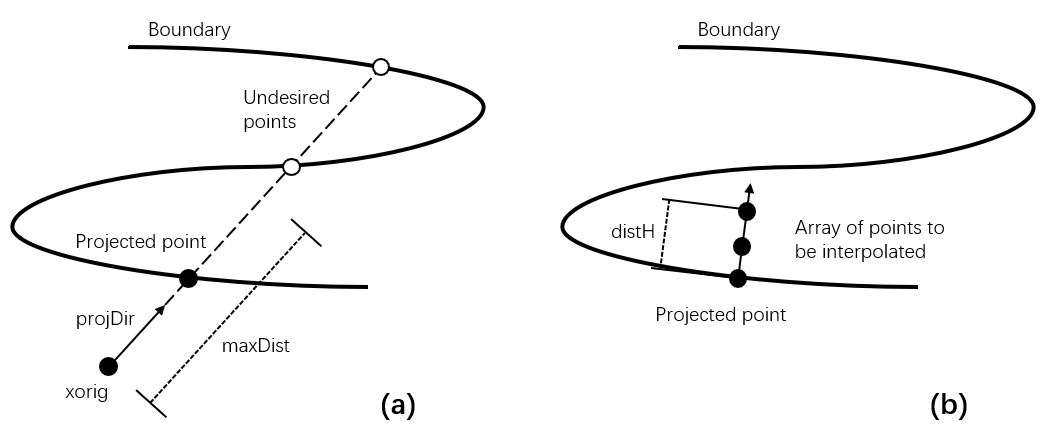
\includegraphics[width = 0.9 \textwidth]{img/module_wallNormalData.jpg}
    \caption{(a) Project the input point onto the boundary, (b) Array of 
    points to be interpolated.}
  \end{center}
\end{figure}
%
%
%

\subsection{Manipulating meshes with FieldConvert}
FieldConvert has support for two modules that can be used in conjunction with
the linear elastic solver, as shown in chapter~\ref{s:elasticity}. To do this,
FieldConvert has an XML output module, in addition to the Tecplot and VTK
formats.

The \inltt{deform} module, which takes no options, takes a displacement field
and applies it to the geometry, producing a deformed mesh:
\begin{lstlisting}[style=BashInputStyle]
FieldConvert -m deform input.xml input.fld deformed.xml
\end{lstlisting}

The \inltt{displacement} module is designed to create a boundary condition field
file. Its intended use is for mesh generation purposes. It can be used to
calculate the displacement between the linear mesh and a high-order surface, and
then produce a \inltt{fld} file, prescribing the displacement at the boundary,
that can be used in the linear elasticity solver.

Presently the process is somewhat convoluted and must be used in conjunction
with NekMesh to create the surface file. However the bash input below
describes the procedure. Assume the high-order mesh is in a file called
\inlsh{mesh.xml}, the linear mesh is \inlsh{mesh-linear.xml} that can be
generated by removing the \inltt{CURVED} section from \inlsh{mesh.xml}, and that
we are interested in the surface with ID 123.

\begin{lstlisting}[style=BashInputStyle]
# Extract high order surface
NekMesh -m extract:surf=123 mesh.xml mesh-surf-curved.xml

# Use FieldConvert to calculate displacement between two surfaces
FieldConvert -m displacement:id=123:to=mesh-surf-curved.xml \
    mesh-linear.xml mesh-deformation.fld

# mesh-deformation.fld is used as a boundary condition inside the
# solver to prescribe the deformation conditions.xml contains
# appropriate Nektar++ parameters (mu, E, other BCs, ...)
LinearElasticSolver mesh-linear.xml conditions.xml

# This produces the final field mesh-linear.fld which is the
# displacement field, use FieldConvert to apply it:
FieldConvert-g -m deform mesh-linear.xml mesh-linear.fld mesh-deformed.xml
\end{lstlisting}

\section{FieldConvert in parallel}
To run FieldConvert in parallel the user needs to compile
\nekpp with MPI support and can employ the following
command
\begin{lstlisting}[style=BashInputStyle]
mpirun -np <nprocs> FieldConvert test.xml test.fld test.dat
\end{lstlisting}
\begin{lstlisting}[style=BashInputStyle]
mpirun -np <nprocs> FieldConvert test.xml test.fld test.plt
\end{lstlisting}
or
\begin{lstlisting}[style=BashInputStyle]
mpirun -np <nprocs> FieldConvert test.xml test.fld test.vtu
\end{lstlisting}
replacing \inltt{<nprocs>} with the number of processors. For the
\inltt{.dat} and \inltt{.plt} outputs the current version will proudce
a single output file.  However it is also sometimes useful to produce
multiple output files, one for each partition, and this
can be done by using the \inltt{writemultiplefiles} option, i.e.
\begin{lstlisting}[style=BashInputStyle]
  mpirun -np <nprocs> FieldConvert test.xml test.fld \
                  test.dat:dat:writemultiplefiles
\end{lstlisting}
\begin{lstlisting}[style=BashInputStyle]
  mpirun -np <nprocs> FieldConvert test.xml test.fld \
                  test.plt:plt:writemultiplefiles
\end{lstlisting}

For the \inltt{.vtu} format multiple files will by default be produced
of the form \inltt{test\_vtu/P0000000.vtu}, {test\_vtu/P0000001.vtu},
{test\_vtu/P0000002.vtu}. For this format an additional file called
\inltt{test.pvtu} is written out which allows for parallel reading of the
individual \inltt{.vtu} files.

FieldConvert functions that produce a \inltt{.fld} file output will
also be created when running in parallel. In this case when producing
a .fld file a directory called \inltt{test.fld} (or the specified
output name) is created with the standard parallel field files placed
within the directory.
%
%
%
\section{Processing large files in serial}
When processing large files, it is not always convenient to run in parallel but
process each parallel partition in serial, for example when interpolating a
solution field from one mesh to another or creating an output file for
visualization.


\subsection{Using the \textit{ part-only} and \textit{ part-only-overlapping} options}

Loading full \inltt{file1.xml} can be expensive if the
\inltt{file1.xml} is already large. So instead you can pre-partition
the file using the using the \inltt{--part-only} option. So the
command
\begin{lstlisting}[style=BashInputStyle]
FieldConvert --part-only 10 file.xml file.fld
\end{lstlisting}
will partition the mesh into 10 partitions and write each partition into a
directory called \inltt{file\_xml}. If you enter this directory you will find
partitioned XML files \inltt{P0000000.xml}, \inltt{P0000001.xml}, \dots,
\inltt{P0000009.xml} which can then be processed individually as outlined above.

There is also a \inltt{--part-only-overlapping} option, which can be run in the
same fashion.
\begin{lstlisting}[style=BashInputStyle]
FieldConvert --part-only-overlapping 10 file.xml file.fld
\end{lstlisting}
In this mode, the mesh is partitioned into 10 partitions in a similar manner,
but the elements at the partition edges will now overlap, so that the
intersection of each partition with its neighbours is non-empty. This is
sometime helpful when, for example, producing a global isocontour which has been
smoothed. Applying the smoothed isocontour extraction routine with the
\inltt{--part-only} option will produce a series of isocontour where there will
be a gap between partitions, as the smoother tends to shrink the isocontour
within a partition. using the \inltt{--part-only-overlapping} option will still
yield a shrinking isocontour, but the overlapping partitions help to overlap the
partiiton boundaries.

\subsection{Using the \textit{nparts} options}

If you have a partitioned directory either from a parallel run or
using the \inltt{--part-only} option you can now run the
\inltt{FieldConvert} option using the \inltt{nparts}  command line
option, that is
\begin{lstlisting}[style=BashInputStyle]
FieldConvert --nparts 10  file1\_xml:xml file1.fld file1.vtu
\end{lstlisting}

Note the form \inltt{file1\_xml:xml} option tells the code it is a
parallel partition which should be treated as an \inltt{xml} type
file. the argument of \inltt{nparts} should correpsond to the number
of partitions used in generating the file1\_xml directory. This will
create a parallel vtu file as it processes each partition.


Another example is to interpolate \inltt{file1.fld} from one mesh
\inltt{file1.xml} to another \inltt{file2.xml}. If the mesh files are
large we can do this by partitioning \inltt{file2.xml} into 10 (or
more) partitions to generate the \inltt{file\_xml} directory and
interpolating each partition one by one using the command:
\begin{lstlisting}[style=BashInputStyle]
  FieldConvert --nparts 10 -m interpfield:fromxml=file1.xml:fromfld=file1.fld \
  file2_xml:xml file2.fld
\end{lstlisting}
Note that internally the routine uses the range option so that it only
has to load the part of \inltt{file1.xml} that overlaps with each
partition of \inltt{file2.xml}.  The resulting output will lie in a
directory called \inltt{file2.fld}, with each of the different
parallel partitions in files with names \inltt{P0000000.fld},
\inltt{P0000001.fld}, \dots, \inltt{P0000009.fld}. In previous
versions of FieldConvert it was necessary to generate an updated
\inltt{Info.xml} file but in the current version it should
automatically be updating this file.

\subsection{Running in parallel with the \textit{ nparts} option}

The examples above will process each partition serially which may now
take a while for many partitions. You can however run this option in
parallel using a smaller number of cores than the nparts.

For the example of creating a vtu file above you can use 4 processor
concurrently wiht the command line:
\begin{lstlisting}[style=BashInputStyle]
mpirun -n 4 FieldConvert --nparts 10   file1\_xml:xml file1.fld file1.vtu
\end{lstlisting}

Obviously the executable will have to have been compiled with the MPI
option for this to work.


%%% Local Variables:
%%% mode: latex
%%% TeX-master: "../user-guide"
%%% End:
